\documentclass[11pt,a4paper]{article}
\usepackage{graphicx}
\usepackage{amsmath}
\usepackage{geometry}
\geometry{margin=1in}
\graphicspath{{../}}

\title{Assignment 2: Flow Over a Cylinder}
\author{Sajeev}
\date{September 2025}

\begin{document}
\maketitle

\section{Governing Equations \& Setup}
The unsteady, 2D incompressible flow over a cylinder is simulated by solving the transient Continuity and Navier-Stokes equations. 
Simulations were conducted at $Re=272$ (Laminar) and $Re=2902$ (Standard $k-\epsilon$ turbulence model). The SIMPLE algorithm, QUICK momentum scheme, and 2nd Order Implicit transient formulation were employed with a convergence target of $10^{-6}$. 

\section{Flow Fields \& Vortex Shedding}
A block-structured grid with high refinement near the cylinder was used to capture boundary layer separation. 
At $Re=272$, the flow separates behind the cylinder, forming a distinct, alternating Von Kármán vortex street in the wake. 
However, at $Re=2902$ using the Standard $k-\epsilon$ model, the vortex shedding is almost completely damped out, resulting in a steady, smeared, symmetric wake. This is a known limitation of the standard $k-\epsilon$ RANS formulation, which generates excessive turbulent viscosity in wake regions, suppressing the physical instabilities.

\begin{figure}[h!]
    \centering
    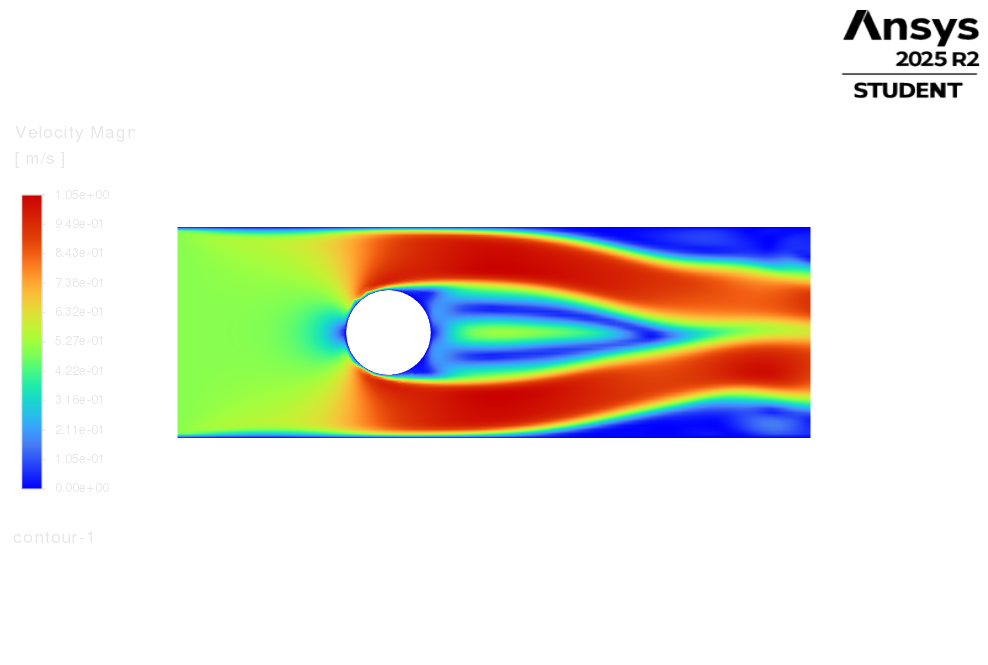
\includegraphics[width=0.48\linewidth]{vel-contour-272-2000.png}
    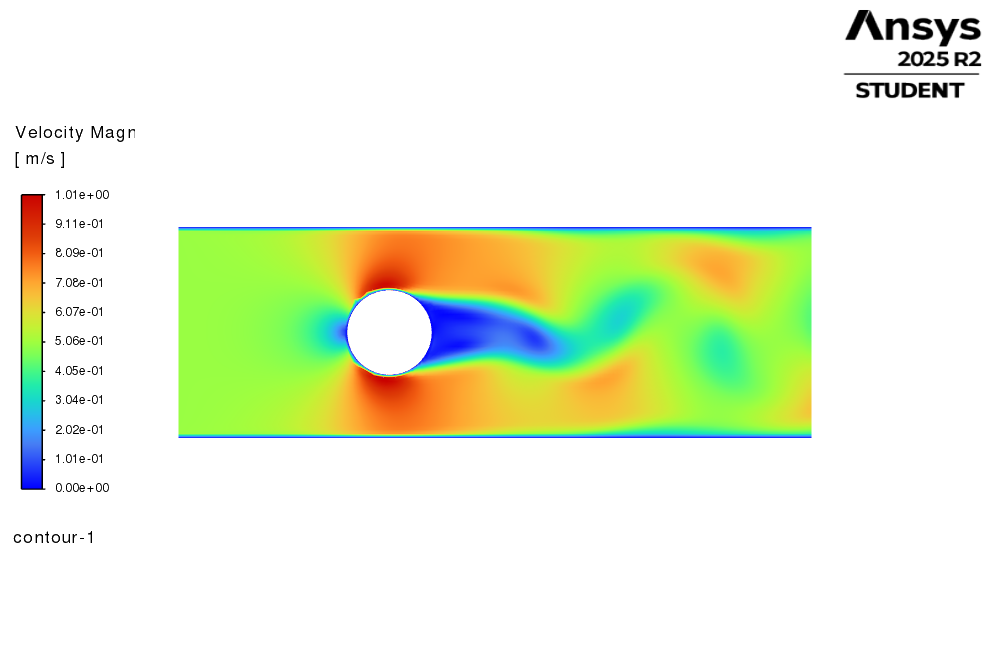
\includegraphics[width=0.48\linewidth]{vel-contour-2902-2000.png}
    \caption{Velocity contours. Left: $Re=272$ (Laminar). Right: $Re=2902$ (Standard $k-\epsilon$).}
\end{figure}

\section{Frequency Analysis}
Monitoring the $y$-velocity in the wake over time allowed for frequency analysis. For $Re=272$, the oscillation period $T$ from the probe data was approximately $11$ s, yielding a shedding frequency $f \approx 0.091$ Hz. This perfectly aligns with the analytical expected Strouhal number $St = fD/U \approx 0.183$ (which predicts $f = 0.183 \times 0.5 / 1 = 0.0915$ Hz). Conversely, the turbulent simulation ($Re=2902$) showed damped probe data, failing to capture the physical shedding frequency unless more advanced models (e.g., RSM, LES) are used.

\end{document}
